\section{Contextual Design Modelle}\label{sec:modelle}

Contextual Design Modelle sollen die Erfassung des Kontextes weiter vereinfachen.
Hierzu gibt es eine Vielzahl verschiedener Modelltypen.
Diese können digital, aber auch physisch vorliegen.
Auch können verschiedene Modelltypen kombiniert werden.
Im Folgenden seien die in \cite{NOG} besprochenen Modelltypen aufgelistet und kurz beschrieben.
Zu diesen sind jeweils Beispiele aus der Gebäudetechnik der Universität Bremen gegeben.
Diese sind \cite{NOG} entnommen.

\subsection{Flussmodell}

Ein Flussmodell ist als ein gerichteter Graph zu verstehen.
Dabei sind die Knoten Gegenstände, Räume oder Personen.
Die Kanten stellen Tätigkeiten oder andere Leistungen der Objekte dar.
Knoten können in ihrer Darstellung variabel sein
Beispielsweise können Personen als Ellipsen und Räume als Rechtecke dargestellt werden.

\begin{figure}[htp]
    \centering
    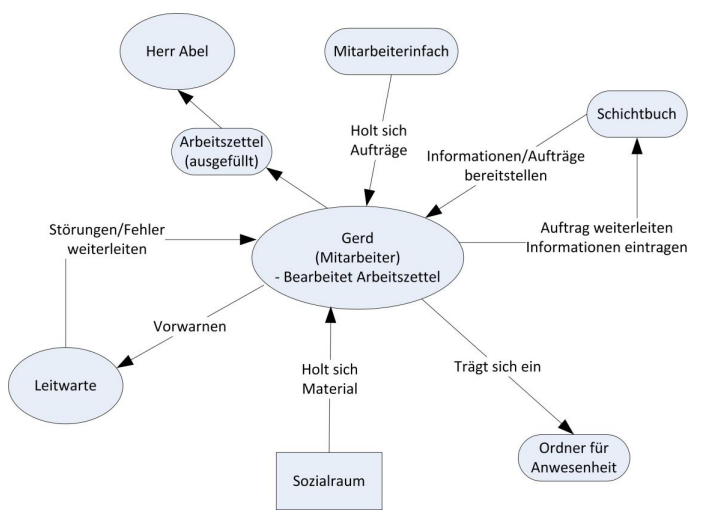
\includegraphics[width=.7\textwidth]{images/3-Modelle/flussmodell.png}
    \caption{Beispiel Flussmodell aus \cite{NOG}}
    \label{fig:flussmodell}
\end{figure}

\autoref{fig:flussmodell} die Abläufe der Gebäudetechnik der Universität Bremen als Flussmodell.
Aus einem Flussmodell sind schnell grobe Abläufe und Abhängigkeiten zu erkennen.
Dies ist nützlich, wenn ein Bild des gesamten Kontextes benötigt wird.
Informationen sind hier jedoch abstrakt und nicht konkret an einem Beispielszenario gezeigt.
Es ist also zu empfehlen, zusätzlich zu einem Flussmodell ein weiteres, konkretes Modell heranzuziehen.

\subsection{Sequenzmodell}

Sequenzmodelle stellen konkrete Abläufe in detaillierten atomaren Schritten dar.
Dabei wird zu jedem Schritt ein Zweck, die Handlung und mögliche Störfälle notiert.
Sequenzmodelle können auch die Erfahrungen mehrerer Ausführungen einer Tätigkeit enthalten.
Dies ist im in \autoref{fig:sequenzmodell} zu sehenden Modell der Fall.

\begin{figure}[htp]
    \centering
    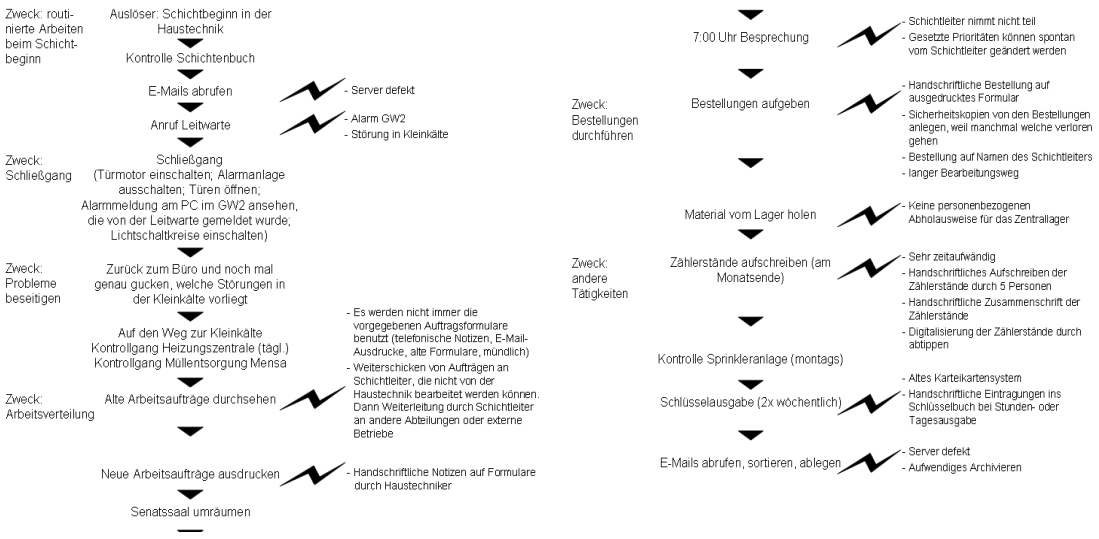
\includegraphics[width=\textwidth]{images/3-Modelle/sequenzmodell.png}
    \caption{Beispiel Sequenzmodell aus \cite{NOG}}
    \label{fig:sequenzmodell}
\end{figure}

In diesem wurde ein Haustechniker mehrere Tage bei seiner morgendlichen Routine begleitet.
Die daraus gewonnenen Eindrücke und Informationen wurden mit Hilfe eines Sequenzmodells dargestellt.
Dieses Modell ist nützlich, wenn konkrete Abläufe detailliert betrachtet werden sollen.
Es eignet sich jedoch nicht, um einen größeren Kontext in seiner Gesamtheit zu erfassen.

\subsection{Kulturelles Modell}

Kulturelle Modelle spiegeln das soziale Umfeld des Kontextes wider.
Es ist ähnlich wie ein Flussmodell aufgebaut.
Die Kanten stehen nun jedoch für kulturelle und soziale Ansichten.
Diese können auch in Form von Zitaten an die Kanten geschrieben werden.
Ebenso ist es möglich, mehrere Ansichten an einer Kante anzufügen.

Kulturelle Modelle sind geeignet, damit der soziale Kontext der Kontextpersonen betrachtet werden kann.
Es hilft, wenn Beziehungen zwischen verschiedenen Individuen im Kontext untersucht werden sollen.

\subsection{Physikalisches Modell}

Physikalische Modelle spiegeln den räumlichen Kontext wider.
Aus ihnen ist zu erkennen in welchem Gebiet und Umfang sich die Nutzenden während der Ausführung ihrer Aufgaben bewegen müssen.
Diese Modelle können im zweidimensionalen Raum, aber auch als dreidimensionale Modelle ausgeführt werden.
Wichtig ist jedoch, dass die Wege oder Arbeitsplätze der Nutzenden aus diesen Modellen erkenntlich sind.
Nicht erweiterte Grundrisse stellen hier kein echtes physikalisches Modell dar.

\begin{figure}[htp]
    \centering
    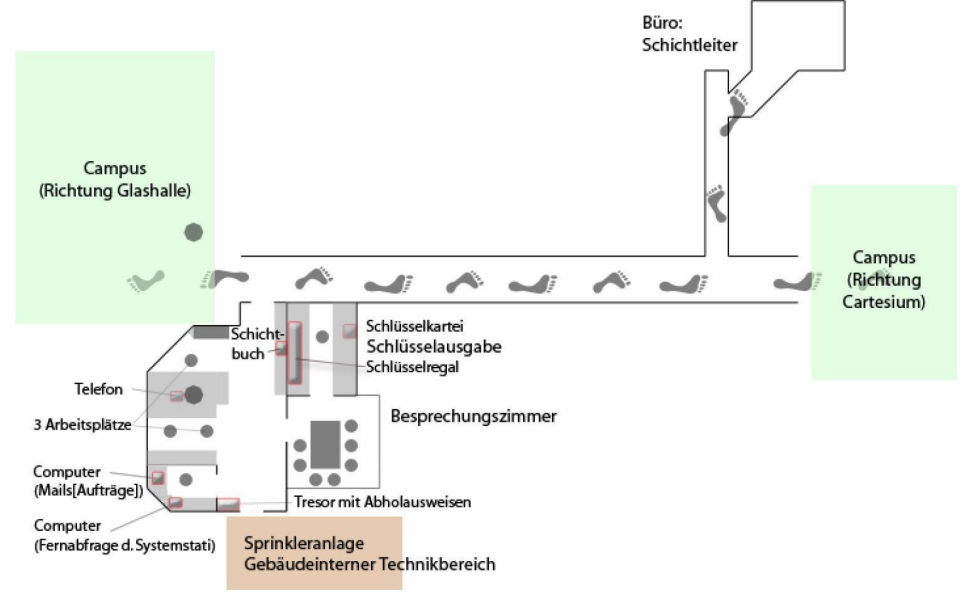
\includegraphics[width=.75\textwidth]{images/3-Modelle/physikalischesmodell.png}
    \caption{Beispiel Physikalisches Modell aus \cite{NOG}}
    \label{fig:physikalischesModell}
\end{figure}

\autoref{fig:physikalischesModell} zeigt ein physikalisches Modell der Aufgaben eines Haustechnikers der Universität Bremen.
Aus ihm sind sowohl der Arbeitsplatz der Haustechniker, also auch deren Wege im Gebäude ersichtlich.
Darüber hinaus wurden wichtige Orte und Objekte in der zweidimensionalen Ansicht markiert.

\subsection{Artefaktmodell}

Als Artefaktmodelle sind sämtliche Dokumente oder Gegenstände benannt, welche dem Nutzungskontext entstammen.
Sie helfen, wenn der Einsatz von Medien genauer untersucht werden soll.
Im Falle der Haustechnik kann hier beispielsweise ein Schichtbuch oder eine Schlüsselkarte, welche das Ausleihen von Schlüsseln dokumentiert, herangezogen werden.
Artefaktmodelle werden im Gegensatz zu den bisher kennengelernten Modellen nicht von den Entwickelnden, sondern von den Nutzenden erstellt und zur Verfügung gestellt.

\subsection{Culture Probes}

Culture Probes können ähnlich wie Artefaktmodelle gesehen werden, werden jedoch nicht vorgefunden, sondern wissentlich von den Nutzenden erstellt.
Hierzu werden den Nutzenden Hilfsmittel zur Verfügung gestellt, mit denen sich während der Ausführung ihrer Tätigkeiten agieren können.
Hier kann es sich um Zettel und Stift, aber auch eine Kamera handeln.

Bei der Auswertung von Culture Probes ist entstandenes Material nach Tätigkeiten zu Gruppieren.
Es ist somit wichtig, dass erkenntlich ist, aus welcher Tätigkeit ein erstelltes Artefakt entstammt.